\documentclass[conference]{IEEEtran}
\IEEEoverridecommandlockouts
\usepackage{newtxtext,newtxmath}
\usepackage{cite}
\usepackage{amsmath}
\usepackage{algorithmic}
\usepackage{booktabs}
\usepackage{array}
\usepackage{graphicx}
\usepackage{tikz}
\usetikzlibrary{arrows.meta,positioning,fit,calc,backgrounds}
\usepackage{url}
\usepackage{xcolor}
\usepackage{enumitem}
\setlist{nosep,leftmargin=*}
\setlength{\textfloatsep}{6pt plus 1pt minus 2pt}
\setlength{\floatsep}{5pt plus 1pt minus 2pt}
\setlength{\emergencystretch}{1em}
\setlength{\intextsep}{5pt plus 1pt minus 2pt}
\renewcommand{\arraystretch}{1.05}
\hyphenation{Data-Guard Iso-la-tion Run-book tele-me-try}

\begin{document}

\title{DataGuard AI: Visual Telemetry Fingerprinting and Risk-Governed Agentic Data-Quality Incident Response}

\author{\IEEEauthorblockN{Tishya Jha}
\IEEEauthorblockA{Department of Computer Science and Design Engineering\\
Rajiv Gandhi Institute of Petroleum Technology\\
\texttt{23cd3049@rgipt.ac.in}}
\and
\IEEEauthorblockN{Aarna Kumar}
\IEEEauthorblockA{Department of Computer Science and Design Engineering\\
Rajiv Gandhi Institute of Petroleum Technology\\
\texttt{23cd3001@rgipt.ac.in}}}

\maketitle

\begin{abstract}
Data pipelines may finish successfully while emitting incomplete, duplicated, schema-incompatible, or distribution-shifted outputs. DataGuard AI is an implemented local Python modular monolith connecting structured quality checks, Isolation Forest, evidence-grounded root-cause analysis (RCA), local runbook retrieval, guarded simulated actions, verification, persistence, FastAPI, and an API-backed Streamlit dashboard. Its digital image processing module encodes a Data Quality Fingerprint (DQF), with a separate validity mask for missing telemetry, and maps OpenCV regions back to run and metric identifiers. On the reproducible 360-run synthetic benchmark, the 72-run test split produced F1=0.800 for the severity baseline and F1=0.732 (AP=0.591) for structured Isolation Forest. On a matched 43-run subset, adding DQF-region features raised F1 from 0.789 to 0.862 while AP fell from 0.764 to 0.673. Across three held-out fingerprints (1,024 valid pixels), global Otsu segmentation reached F1=0.779 and IoU=0.638; the adaptive/morphological alternative scored 0.324 and 0.194. Fixed local evaluations measured runbook hit@3 at 6/7 and RCA top-1/top-3 accuracy at 4/5 and 5/5. These synthetic results demonstrate a working prototype and also expose its limitations.
\end{abstract}

\begin{IEEEkeywords}
Data quality, anomaly detection, digital image processing, root-cause analysis, retrieval-augmented generation, human-in-the-loop systems.
\end{IEEEkeywords}

\section{Introduction}
Data reliability cannot be inferred from process completion alone: a successful pipeline execution may still introduce null surges, duplicate keys, row-count drops, schema drift, or population shifts. Such failures propagate through dependent datasets and can remain latent until downstream analytics are affected. Rule-based checks are interpretable but often leave operators to correlate telemetry, schema history, lineage, prior incidents, and remediation outcomes manually. A reliable incident-response system must preserve evidence, distinguish observations from causal hypotheses, control state-changing actions, and verify the post-action state rather than merely generate an explanation.

DataGuard AI implements this closed loop in one Python modular monolith: normalised telemetry feeds structured quality checks and anomaly detection; DQF regions add visual evidence; RCA combines findings with schema, lineage, and history; runbook retrieval informs a typed plan; and a server-side policy guard gates action before verification and persistence.

The contributions are an auditable pixel-to-telemetry encoding with explicit missingness, a comparative classical-DIP pipeline, a single orchestrator with typed tools and mandatory approval for high-risk actions, and an evaluation spanning detection, segmentation, retrieval, tool safety, and latency. The system is evaluated on a seeded synthetic benchmark; its results and limitations are reported in Section V.

\section{Related Work and State of the Art}
Automated data-quality systems combine declarative constraints, historical metrics, and anomaly detection~\cite{deequ}; Isolation Forest provides an efficient unsupervised score through random partitioning~\cite{isolation}. Recent image-encoded time-series work uses learned representations to localise sensor anomalies~\cite{ma2024}. DataGuard AI instead uses a calibrated DQF with classical OpenCV operators and retains structured findings as the authoritative quality evidence.

Image encodings have been used for time-series inspection and classification~\cite{wang}; Otsu thresholding supplies a global baseline~\cite{otsu}, and morphology analyses foreground shape~\cite{serra}. DQF interpretation requires stable intensity calibration, channel order, missingness, and pixel-to-telemetry mapping. Accordingly, the evaluation scores saved masks against injected-defect labels rather than treating a dashboard heatmap as evidence by itself.

Retrieval-augmented generation grounds generated responses in retrieved passages~\cite{rag}, while reasoning-and-acting research motivates iterative evidence collection and action selection~\cite{react}. For guarded remediation, however, a language model must not execute arbitrary code or override policy. DataGuard AI narrows these ideas into a single state machine, source-cited runbook retrieval, explicit tool contracts, server-side approval checks, and post-action verification. The research gap addressed is the integration of structured quality checks, visual evidence, evidence-grounded RCA, runbook references, risk-governed action, and persisted outcome verification in one reproducible local prototype.

\section{Proposed Methodology and Architecture}
\subsection{Modular Closed-Loop Design}
The system follows four dependency layers: domain contracts, application use cases, infrastructure adapters, and presentation. Ingestion and normalisation have one owner; \texttt{quality.py} evaluates rules once; a canonical feature builder supplies a stable named vector; \texttt{visual\_inspection.py} owns DQF encoding and DIP; detection and incident services deduplicate findings; RCA ranks hypotheses; RAG owns chunking and retrieval; and a single \texttt{AgentOrchestrator} owns state transitions. FastAPI exposes application use cases, whereas Streamlit acts only as an API client. SQLite stores relational entities and audit events; image arrays and rendered artifacts are stored as files with stable relative references.

\begin{figure*}[t]
\centering
\resizebox{0.94\textwidth}{!}{%
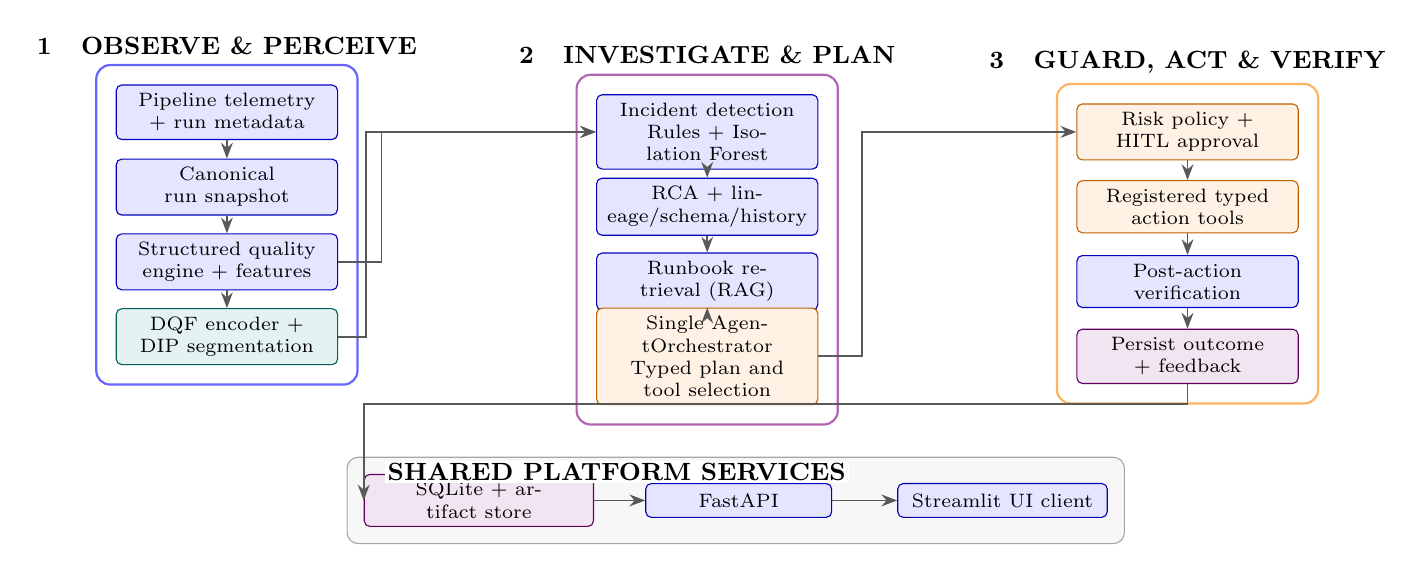
\begin{tikzpicture}[
  font=\scriptsize,
  arr/.style={-{Stealth[length=2mm]},draw=black!65,line width=0.65pt},
  card/.style={draw=#1!75!black,fill=#1!10,rounded corners=2pt,align=center,text width=2.60cm,minimum height=0.52cm,inner sep=3pt},
  group/.style={draw=#1!60,rounded corners=5pt,line width=0.8pt,inner sep=7pt},
  node distance=0.20cm and 0.32cm
]
% left pipeline (fixed coordinates keep the diagram legible at conference scale)
\node[card=blue] (tele) at (1.55,4.45) {Pipeline telemetry + run metadata};
\node[card=blue] (canon) at (1.55,3.50) {Canonical run snapshot};
\node[card=blue] (quality) at (1.55,2.55) {Structured quality engine + features};
\node[card=teal] (dqf) at (1.55,1.60) {DQF encoder + DIP segmentation};
\node[group=blue,fit=(tele)(canon)(quality)(dqf),label={[font=\small\bfseries]above:1\quad OBSERVE \& PERCEIVE}] (g1) {};
% middle pipeline
\node[card=blue] (det) at (7.65,4.20) {Incident detection\\Rules + Isolation Forest};
\node[card=blue] (rca) at (7.65,3.25) {RCA + lineage/schema/history};
\node[card=blue] (rag) at (7.65,2.30) {Runbook retrieval (RAG)};
\node[card=orange] (orch) at (7.65,1.35) {Single AgentOrchestrator\\Typed plan and tool selection};
\node[group=violet,fit=(det)(rca)(rag)(orch),label={[font=\small\bfseries]above:2\quad INVESTIGATE \& PLAN}] (g2) {};
% right pipeline
\node[card=orange] (policy) at (13.75,4.20) {Risk policy + HITL approval};
\node[card=orange] (tools) at (13.75,3.25) {Registered typed action tools};
\node[card=blue] (verify) at (13.75,2.30) {Post-action verification};
\node[card=violet] (outcome) at (13.75,1.35) {Persist outcome + feedback};
\node[group=orange,fit=(policy)(tools)(verify)(outcome),label={[font=\small\bfseries]above:3\quad GUARD, ACT \& VERIFY}] (g3) {};
% cross-stage arrows
\draw[arr] (tele) -- (canon);
\draw[arr] (canon) -- (quality);
\draw[arr] (quality) -- (dqf);
\draw[arr] (quality.east) -- ++(0.55,0) |- (det.west);
\draw[arr] (dqf.east) -- ++(0.35,0) |- (det.west);
\draw[arr] (det) -- (rca);
\draw[arr] (rca) -- (rag);
\draw[arr] (rag) -- (orch);
\draw[arr] (orch.east) -- ++(0.55,0) |- (policy.west);
\draw[arr] (policy) -- (tools);
\draw[arr] (tools) -- (verify);
\draw[arr] (verify) -- (outcome);
% shared services at bottom
\node[card=violet,text width=2.7cm,minimum height=0.43cm] (db) at (4.75,-0.48) {SQLite + artifact store};
\node[card=blue,text width=2.15cm,minimum height=0.43cm] (api) at (8.05,-0.48) {FastAPI};
\node[card=blue,text width=2.45cm,minimum height=0.43cm] (ui) at (11.4,-0.48) {Streamlit UI client};
\begin{scope}[on background layer]
\node[draw=black!35,fill=black!3,rounded corners=4pt,fit=(db)(api)(ui),inner sep=6pt] (platform) {};
\end{scope}
\node[font=\small\bfseries,anchor=west,fill=white,inner sep=1pt] at (3.55,-0.12) {SHARED PLATFORM SERVICES};
\draw[arr] (db) -- (api);
\draw[arr] (api) -- (ui);
\draw[arr] (outcome.south) -- ++(0,-0.25) -| (db.west);
\end{tikzpicture}}
\caption{DataGuard AI architecture. The DQF/DIP channel contributes mapped evidence to detection and investigation; structured quality rules remain authoritative. All state-changing actions pass through policy and typed tools before verification and persistence.}
\label{fig:architecture}
\end{figure*}

\subsection{Canonical Quality Evidence and Detection}
Ingestion validates timestamps, row counts, duration, schema version, source/target identifiers, and field-level metrics, then creates one canonical run snapshot. The quality engine performs six classes of checks: null/missing rates, duplicate-key rates, input/output row-count deltas, schema additions/removals/renames/type changes, invalid type/range/value checks, and numerical distribution deviation. Each finding records its rule ID, severity, observed and expected values, evidence, and timestamp. The feature builder creates a stable named vector from run telemetry and findings. A deterministic threshold baseline is compared with an Isolation Forest model; its anomaly score is not interpreted as a calibrated probability. Training, validation, and test partitions are grouped chronologically or by incident, and the decision threshold is selected on validation data and frozen before testing.

\subsection{Data Quality Fingerprint and DIP}
For a fixed history window, DQF rows correspond to ordered runs and columns to a versioned list of $(\text{field\_id},\text{metric\_id})$ channels. Let $x_{r,c}$ be a metric, $m_c$ its healthy reference (e.g., the training median), and $s_c$ a robust channel scale (e.g., the median absolute deviation) estimated from training data. Its calibrated deviation and 8-bit intensity are
\begin{equation}
 d_{r,c}=\min\!\left(1,\frac{|x_{r,c}-m_c|}{\kappa s_c+\epsilon}\right),\quad I_{r,c}=\operatorname{round}(255d_{r,c}),
\end{equation}
where $\kappa$ and $\epsilon$ are configured. Channel order, baseline version, image dimensions, run IDs, and channel IDs are persisted. A validity mask $M\in\{0,1\}^{W\times C}$ distinguishes missing observations from low risk.

The implemented DIP-B0 applies Otsu global thresholding and connected-component analysis. DIP-P1 uses adaptive thresholding, a $3\times3$ elliptical morphological closing, and connected-component analysis; median filtering is disabled because the generator adds no impulse noise. Each region records area, bounding box, centroid, temporal/channel spans, peak intensity, density, and mapped run/metric IDs. The evaluated DQF is $30\times12$ with adaptive block size 11 and offset $-2$. Encoder metadata, configuration, intermediate images, masks, overlays, and region CSVs are persisted with each artifact.

\noindent\textbf{DIP procedure:} (1) encode the chronological window and validity mask; (2) produce DIP-B0 and DIP-P1 masks; (3) label connected regions and map coordinates to source run/channel IDs; (4) save the raw image, masks, overlay, region table, configuration, and processing duration; (5) compare both methods against injected-defect masks using precision, recall, F1, and IoU or Dice. Three configured DQF-region features (maximum persistence, region density, and affected-channel count) were included in a matched held-out detector ablation. A segmented region is evidence of a pattern, not proof of causation.

\subsection{Investigation, Retrieval, and Guarded Action}
RCA ranks hypotheses from quality findings, schema diffs, dependency lineage, recent runs, historical incidents, action outcomes, and optional DQF regions. A row-count drop paired with an upstream failure supports an upstream-dependency hypothesis; a type mismatch aligned with a schema change supports schema drift. Conflicting or sparse evidence yields \texttt{INCONCLUSIVE} rather than a fabricated cause.

Seven local Markdown runbooks are chunked with stable source IDs and retrieved by deterministic TF--IDF cosine similarity. Retrieved chunks retain document ID, section ID, score, and source text. A single \texttt{AgentOrchestrator} controls transitions \texttt{NEW}$\rightarrow$\texttt{INVESTIGATING}$\rightarrow$\texttt{PROPOSED}, followed by approval or execution readiness, \texttt{EXECUTING}, and \texttt{VERIFYING}, ending in \texttt{RESOLVED}, \texttt{ESCALATED}, or \texttt{FAILED}. Each typed plan includes tool, arguments, preconditions, evidence/runbook references, risk, and expected outcome.

The allowlist includes read-only inspection and retrieval, reversible quarantine, simulated rerun, sandboxed simulated repair, and escalation. Quarantine is idempotent; reruns do not invoke a real scheduler; repairs preserve the original artifact. Ambiguous or high-risk actions require an explicit approval record, checked server-side at execution time. Each transition and tool result is audited with correlation and incident IDs. Verification reruns the relevant checks; failed verification leaves the incident unresolved or escalates it.

\begin{algorithmic}[1]
\STATE Validate telemetry; persist the canonical run and compute quality findings/features
\STATE Encode DQF; run DIP-B0/DIP-P1; persist masks and mapped regions
\STATE Detect and deduplicate the incident; rank evidence-backed RCA hypotheses and retrieve cited runbook sections
\STATE Build a typed plan; enforce tool allowlist, preconditions, risk policy, and required approval
\STATE Execute the local/simulated action; re-check quality and persist verification, audit trace, and outcome
\end{algorithmic}

\section{Implementation and Experimental Setup}
DataGuard AI is implemented and runnable as a Python modular monolith. Modules cover strict JSONL ingestion and synthetic data generation, schema/lineage, one structured quality engine, canonical features, DQF encoding and OpenCV processing, Isolation Forest and severity-baseline scoring, incident deduplication, evidence-ranked RCA, TF--IDF runbook retrieval, a single orchestration state machine, typed action tools and server-side approval, post-action checks, SQLite JSON-record persistence, FastAPI routes, Streamlit screens, and saved evaluation artifacts. Runtime dependencies are NumPy, OpenCV, scikit-learn, FastAPI, Pydantic Settings, Streamlit, Uvicorn, and Joblib; Python's standard-library SQLite driver handles persistence. YAML and environment configuration own thresholds, model parameters, DIP settings, approval policy, database paths, and artifact paths.

Eight registered tool operations provide inspection, retrieval, quarantine/release, simulated rerun, schema-alignment simulation, escalation, and approval recording. FastAPI exposes health, demo generation, run inspection/analysis, incident investigation/planning, approval, action execution, timelines, DQF artifact allowlists, and evaluation summaries under \texttt{/api/v1}. SQLite persists runs, findings, incidents, approvals, state transitions, tool audits, action outcomes, and artifact references; images and masks remain files with stable references. Streamlit is an API-only client with five views: overview, DQF processing, incident investigation, actions/approvals, and evaluation. The UI does not duplicate quality rules, inference, or workflow transitions.

Quarantine is idempotent; reruns are local simulations; repairs create a separate schema-aligned artifact and preserve the source. Server-side policy checks preconditions and approval records, and state transitions/tool outcomes are audited. The seeded benchmark contains 360 synthetic runs in 120 incident groups. Grouped partitions contain 216 training runs (24 clean fitting runs), 72 validation runs, and 72 test runs (42 positive, 30 negative). Thresholds are selected on validation and frozen before testing. The DIP experiment evaluates three held-out $30\times12$ fingerprints covering 90 of 108 held-out runs; validity masking leaves 1,024 scored pixels. The matched detection ablation has 43 test runs. AP uses the step-function definition in \url{average_precision_score}, not trapezoidal PR-AUC.

No neural vision network, vector embedding service, production connector, or external scheduler is used. Detection is tree-based; DIP runs through CPU OpenCV; retrieval is local lexical TF--IDF. Saved test outputs include held-out predictions, confusion counts, masks, component metrics, retrieval judgments, RCA cases, and observed timings. Retrieval and RCA medians are measured on the current local environment; no end-to-end production latency or service-level objective is claimed.

\section{Results, Dashboards, and Evaluation}
\subsection{Incident Detection}
Table~\ref{tab:detection} reports held-out scores on the 72-run test partition (42 injected anomalies and 30 non-anomalous runs). The matched DQF-feature ablation improves thresholded F1 and reduces false positives, while average precision declines. No MTTD is reported because the evaluation uses run-level records and has no streaming alert-time protocol.

\begin{table}[t]
\caption{Incident Detection on the Frozen Test Split ($n=72$, 42 Positive Runs)}
\label{tab:detection}
\centering
\footnotesize
\begin{tabular}{@{}lp{0.95in}cccc@{}}
\toprule
\textbf{Configuration} & \textbf{TP/FP/FN/TN} & \textbf{Prec.} & \textbf{Rec.} & \textbf{F1} & \textbf{AP}\\
\midrule
Rule baseline ($n=72$) & 28/0/14/30 & 1.000 & 0.667 & 0.800 & N/A\\
Isolation Forest (structured, $n=72$) & 41/29/1/1 & 0.586 & 0.976 & 0.732 & 0.591\\
Matched IF + DQF regions ($n=43$) & 28/9/0/6 & 0.757 & 1.000 & 0.862 & 0.673\\
\bottomrule
\end{tabular}
\end{table}

\subsection{DIP Segmentation}
Table~\ref{tab:dip} compares global Otsu (DIP-B0) with adaptive thresholding plus morphological closing (DIP-P1) over the same 1,024 valid cells from three held-out masks. DIP-P1 produces substantially more false-positive pixels and regions. Both recover all 90 positive pixels, but DIP-B0 matches 22/23 ground-truth components at IoU $\geq0.5$ while DIP-P1 matches 1/23. Median CPU processing times are measured per $30\times12$ fingerprint.

\begin{table}[t]
\caption{DQF Segmentation on Three Held-Out Fingerprints (1,024 Valid Pixels)}
\label{tab:dip}
\centering
\footnotesize
\begin{tabular}{@{}lccccc@{}}
\toprule
\textbf{Method} & \textbf{Prec.} & \textbf{Rec.} & \textbf{F1} & \textbf{IoU} & \textbf{ms/image}\\
\midrule
DIP-B0: Otsu global & 0.638 & 1.000 & 0.779 & 0.638 & 0.325\\
DIP-P1: adaptive + closing & 0.194 & 1.000 & 0.324 & 0.194 & 0.180\\
\bottomrule
\end{tabular}
\end{table}

\subsection{Agent, Retrieval, and Operational Metrics}
The fixed local retrieval evaluation ranks a relevant runbook section within the top three for 6/7 canonical intent queries (hit@1=hit@3=0.857, MRR=0.857); median measured query time is 0.241 ms and maximum is 0.395 ms. One safe-rerun query is missed, consistent with the lexical retriever's sensitivity to wording. On five evidence-backed synthetic RCA cases, the expected cause is ranked first in 4/5 and appears in the top three in 5/5 (top-1=0.800, top-3=1.000). Median RCA evaluation time is 0.102 ms, with 0.148 ms maximum. Three policy probes (unapproved schema repair, approval by an unauthorized role, and release before verification) were rejected as expected in 3/3 cases; median policy-check time was 0.055 ms (maximum 0.097 ms). These are small fixed-case measurements, not production reliability estimates. Separate integration tests exercise approval gating, source preservation, quarantine, verification, release, restart restoration, and a rerun that remains unresolved when quality defects persist.

The operational judgment sets are deliberately small and handcrafted: seven retrieval queries and five RCA cases. Their measured scores should be read as functional evidence on those cases, not general estimates. No MTTD or end-to-end latency is reported. All benchmark data are synthetic, and the detector test contains only 30 negatives; additional seeds, real labeled incidents, and broader fault distributions are required before making generalization claims.

\subsection{Dashboard and Ablation Interpretation}
The implemented Streamlit UI exposes five views: (1) overview of run volume, failures, and incidents; (2) DQF raw, validity, ground-truth, baseline, adaptive masks and overlays; (3) incident evidence, ranked RCA hypotheses and cited runbook sections; (4) action risk, preconditions, approvals, verification and audit timeline; and (5) evaluation results. Each view consumes FastAPI responses, and simulated actions are labeled. The detection ablation improves F1 at the selected threshold but lowers AP; DQF remains corroborative evidence rather than a causal explanation. The presentation includes captures from the running dashboard.

\section{Conclusion and Future Scope}
DataGuard AI implements a traceable local workflow from canonical telemetry through quality checks and anomaly detection to visual evidence, RCA, runbook retrieval, policy-gated simulated actions, verification, and persisted audit state. On the reproducible synthetic test set, structured Isolation Forest reached F1=0.732 and AP=0.591; adding DQF-region features on a matched subset raised F1 from 0.789 to 0.862 but lowered AP from 0.764 to 0.673. Global Otsu segmentation outperformed the adaptive/morphological alternative in both pixel and region recovery. Retrieval hit@3 was 6/7 and RCA top-3 accuracy 5/5 on fixed small test sets. Results establish that the modular prototype is implemented and runnable, not that it is production ready.

The evidence is limited to synthetic data and small test sets; it does not establish production-scale reliability or generalisation to real incidents. Saved CSV/JSON outputs include held-out predictions and confusion counts, segmentation and region results, per-query retrieval ranks, RCA cases, and observed local timings. Further work should expand seeds and fault amplitudes, independently label production-like incidents, and measure streaming alert time and end-to-end service latency. Neural segmentation and live connectors are outside this local prototype.

\begin{thebibliography}{8}\footnotesize
\bibitem{deequ} S. Schelter \textit{et al.}, ``Automating large-scale data quality verification,'' \emph{Proc. VLDB Endowment}, vol. 11, no. 12, pp. 1781--1794, 2018.
\bibitem{ma2024} J. Ma and H. Wang, ``Anomaly detection in sensor data via encoding time series into images,'' \emph{J. King Saud Univ. Comput. Inf. Sci.}, vol. 36, no. 10, Art. no. 102232, 2024, doi: \url{10.1016/j.jksuci.2024.102232}.
\bibitem{isolation} F. T. Liu, K. M. Ting, and Z.-H. Zhou, ``Isolation forest,'' in \emph{Proc. 8th IEEE Int. Conf. Data Mining (ICDM)}, Pisa, Italy, 2008, pp. 413--422, doi: \url{10.1109/ICDM.2008.17}.
\bibitem{otsu} N. Otsu, ``A threshold selection method from gray-level histograms,'' \emph{IEEE Trans. Systems, Man, and Cybernetics}, vol. SMC-9, no. 1, pp. 62--66, Jan. 1979, doi: \url{10.1109/TSMC.1979.4310076}.
\bibitem{serra} J. Serra, \emph{Image Analysis and Mathematical Morphology}. London, U.K.: Academic Press, 1982.
\bibitem{wang} Z. Wang and T. Oates, ``Encoding time series as images for visual inspection and classification,'' in \emph{Proc. AAAI Workshops}, 2015.
\bibitem{rag} P. Lewis \textit{et al.}, ``Retrieval-augmented generation for knowledge-intensive NLP tasks,'' in \emph{Advances in Neural Information Processing Systems}, vol. 33, pp. 9459--9474, 2020.
\bibitem{react} S. Yao \textit{et al.}, ``ReAct: Synergizing reasoning and acting in language models,'' in \emph{Proc. Int. Conf. Learn. Representations (ICLR)}, 2023.
\end{thebibliography}

\end{document}
